%!TEX root = draft.tex

\section{Simulation and Refinement}
\label{sec:simulation and refinement}



\subsection{Simulation and Refinement}
\label{subsec:simulation and refinement}


{\color {red}In this section, we will give simulation relations $R_{\mathit{sim}}$ between implementation and succinct reference implementation, or reference implementation if the specification is not collection. Such simulation relation will immediate imply history inclusion, and by Theorem \ref{theorem:histories of reference implementation are SRV consistent} and Theorem \ref{theorem:SRIMPSpec and RIMPSpec have same history}, this implies that such implementations are CRVC consistent w.r.t specification.

According to \cite{Abadi:1991,Lynch:1995}, forward simulation is equivalent to refinement provided the right-hand LTS is deterministic. Since the transition labels of $\mathit{Sem}(\mathit{imp})$ and $\mathit{SRImp}(\mathit{Spec})$ are different in message, delivery and arbitration order, $R_{\mathit{sim}}$ needs to do translation between two LTS. To solve this, we model $R_{\mathit{sim}}$ as an relation called $f_s$-simulation, where $f_s$ are used to do translation. We also propose the corresponding refinement $f_t$ of $f_s$-simulation. When $f_s$-simulation and refinement w.r.t $f_t$ satisfies a condition called compatibility, they become equivalent.}

Given two LTS $A_1 = (Q_1,\Sigma_1,\rightarrow_1,q_{0}^1)$ and $A_2 = (Q_2,\Sigma_2,\rightarrow_2,q_{0}^2)$ and two functions $f_s: Q_1 \times Q_2 \times \Sigma_1 \rightarrow \Sigma_2$ and $f_t:\Sigma_1^* \rightarrow \Sigma_2$, we define our simulation and refinement relations as follows:

%Given two LTS $A = (Q_A,\Sigma_A,\rightarrow_A,q_{0A})$ and $B = (Q_B,\Sigma_B,\rightarrow_B,q_{0B})$ with alphabet $\Sigma_A$ and $\Sigma_B$, respectively. Given functions $f_s: Q_A \times Q_B \times \Sigma_A \rightarrow \Sigma_B$ and $f_t:\Sigma_A^* \rightarrow \Sigma_B$, we define our simulation and refinement relations as follows:

%\todo{Use $A_1$ and $A_2$ instead of $A$ and $B$, so that all the components are indexed by 1,2, except for $q_0$ which becomes $q_0^{1/2}$.}

\begin{definition}[$f_s$-Simulation]
\label{definition:fs simulation}
Relation $R \subseteq Q_1 \times Q_2$ is a $f_s$-simulation relation, if whenever $(q_1,q_2) \in R \wedge q_1 {\xrightarrow{\alpha}}_1 q'_1$,
%A $f_s$-simulation relation $R \subseteq Q_A \times Q_B$ is a relation that satisfies: If $(q_a,q_b) \in R \wedge q_a {\xrightarrow{\alpha}}_A q'_a$ for some $q_a$, then
\begin{itemize}
\setlength{\itemsep}{0.5pt}
\item[-] If $f_s(q_1,q_2,\alpha) \neq \epsilon$, then $q_2 {\xrightarrow{f_s(q_1,q_2,\alpha)}}_1 q'_2 \wedge (q'_1,q'_2) \in R$.

\item[-] If $f_s(q_1,q_2,\alpha) = \epsilon$, then $(q'_1,q_2) \in R$.
\end{itemize}
\end{definition}

%\todo{Again, use indexing with 1,2}

\begin{definition}[refinement w.r.t $f_t$]
\label{definition:ft refinement}
$A_2$ refines $A_1$ w.r.t $f_t$, if for each trace $t_1 = \alpha_1 \cdot \ldots \cdot \alpha_k$ of $A_1$, $t_2 = f_t(\alpha_1) \cdot \ldots \cdot f_t(\alpha_1 \cdot \ldots \cdot \alpha_k)$ is an trace of $A_2$.
\end{definition}

%\todo{$B$ $f_t$-refines $A$ to be rewritten to ``$B$ refines $A$ w.r.t. $f_t$''}

%\todo{Give a name to the property $P_{(f_s,f_t)}$, for instance: we say that $f_s$ and $f_t$ are compatible ... }

We say that $f_s$ and $f_t$ are compatible, if for each deterministic $A_2$, the following holds: For each execution %\todo{execution}
$q_{0}^1 {\xrightarrow{\alpha_1}}_1 q_{1}^1 \ldots {\xrightarrow{\alpha_k}}_1 q_{k}^1$ of $A_1$ and each $1 \leq u \leq k$, we have $f_t(\alpha_1 \cdot \ldots \cdot \alpha_{u+1}) = f_s(q_{u}^1,q_{u}^2,\alpha_{u+1})$, here $q_v^2$ is a state obtained by $q_{0}^2 {\xrightarrow{f_t(\alpha_1) \cdot \ldots \cdot f_t(\alpha_1 \cdot \ldots \cdot \alpha_v) }}_2 q_v^2$. %\todo{write it explicitly using the extension of $\xrightarrow{\alpha_1}$ to words}
The following theorem states that if $f_s$ and $f_t$ are compatible, then $f_s$-simulation is equivalent to refinement w.r.t $f_t$. Its proof can be found in Appendix \ref{subsec:proof of theorem equivalence of our simulation and refinement} and is similar to that in \cite{Abadi:1991,Lynch:1995}.

%If $B$ is deterministic, then we defined a property $P_{(f_s,f_t)}$ as follows: For each transitions \todo{execution} $q_{0A} {\xrightarrow{\alpha_1}}$ $q_{1A} \ldots {\xrightarrow{\alpha_k}} q_{kA}$ of $A$, $\forall 1 \leq i < k$, $f_t(\alpha_1 \cdot \ldots \cdot \alpha_i \cdot \alpha_{i+1}) = f_s(q_{iA},q_{iB},\alpha_{i+1})$, where $q_{iB}$ is obtained from $q_{0B}$ by doing $f_t(\alpha_1) \cdot \ldots \cdot f_t(\alpha_1 \cdot \ldots \cdot \alpha_i)$ transitions \todo{write it explicitly using the extension of $\xrightarrow{\alpha_1}$ to words}. The following theorem states that when $P_{(f_s,f_t)}$ holds, $f_s$-simulation is equivalent to $f_t$-refinement. Its proof can be found in Appendix \ref{sec:appendix definitions and proofs of section simulation and refinement} and is similar to that in \cite{Abadi:1991,Lynch:1995}.

\begin{theorem}
\label{theorem:equivalence of our simulation and refinement}
Given an LTS $A_1$ and a deterministic LTS $A_2$ and functions $f_s,f_t$, such that $f_s$ and $f_t$ are compatible. $A_2$ refines $A_1$ w.r.t $f_t$, if and only if there exists a $f_s$-simulation relation between $A_1$ and $A_2$.
\end{theorem}



%\subsection{Collection Specification with Causal Delivery}
\subsection{Example of Simulation Relations}
\label{subsec:collection specification with calusal delivery}

{\color {red}We prove simulation relation for implementations in Table \ref{tab:checked implementations}. Here the first three implementations is more complex and worth consideration. In this subsection, we take the OR-set of \cite{Shapiro:2011} and RGA as example to see that for collection specification with causal delivery, how to construct its simulation relation $R_{\mathit{sim}}$, and how to construct functions $f_s$ and $f_t$ for it.}

\begin{table}[h]
	\centering
	\begin{tabular}{|l|c|c|c|}\hline
		%Implmenentations&\multicolumn{2}{c|}{A4 size paper}\\\hline
        Implmenentations&Assumes causal delivery&Specification&Collection\\\hline
		OR-Set of \cite{Shapiro:2011} &  $\surd$ & OR-set & $\surd$\\
		OR-Set of \cite{Bieniusa:2012} & $\times$ & OR-set & $\surd$\\
        %woot of \cite{Oster:2006} & $\times$ & list & $\surd$\\
        replicated growable array of \cite{Attiya:2016} & $\surd$ & list & $\surd$\\
        counter of \cite{Shapiro:2011} &  $\times$ & counter & $\times$\\
        register of \cite{Shapiro:2011} &  $\times$ & register & $\times$\\\hline
	\end{tabular}
	\caption{Checked Implementations}
	\label{tab:checked implementations}
\end{table}

%Let us take the OR-set algorithms of \cite{Shapiro:2011} as example to define the simulation relation $R_{\mathit{sim}}$.
Given a state $q_{\mathit{imp}} = (\mathit{data},\mathit{msgs},\mathit{msghb})$ of implementation and a state $q_s = (O,\mathit{ro},\mathit{del},\mathit{arb})$ of specification, $(q_{\mathit{imp}},q_s) \in R_{\mathit{sim}}$ normally has the following requirements:

\noindent - A inductive invariants for both $q_{\mathit{imp}}$ and $q_s$. %The inductive invariants normally states some features of local states and operations for executions starting from initial state.

For example: The inductive invariant of $q_{\mathit{imp}}$ requires that (1) For each $\mathit{id} = (r,c)$ in $S \cup \mathit{msgs}$, $c$ is less or equal than counter of replica $r$, and (2) If $(a,S',r,\_)$ is in message, then for each $\mathit{id} \in S'$, $(a,\mathit{id}) \notin \mathit{data}[r].S \wedge (a,\mathit{id},\_,r) \notin \mathit{msgs}$; while The inductive invariants of $q_s$ requires each $\mathit{rem}$ operation is in $\mathit{FstRem}$ of some $\mathit{add}$ operation.

\noindent - A method to check whether an ``$\mathit{add}$ operation'' of $\Sigma_e$ is redundant. If it is, then applying messages of this operation does not change local state.

Example: $(a,\mathit{id})$ is redundant, if for each replica $r$, $(a,\mathit{id}) \notin \mathit{data}[r].S$.

\noindent - A map $f$ between non-redundant elements of $\Sigma_e$ and $O$.%, where $O_s$ is union of $O$ and operations in arbitration order.

Example: $f$ maps $(a,\mathit{id})$ that are not redundant into $\mathit{add}(a)$ and maps $(a,S',r)$ into $\mathit{rem}(a)$. This map preserves replica.

%\noindent - We require that $f(f_{arb}(data,msgs))$ be a sup-sequence of $\mathit{arb}$.

\noindent - There is a message of $x \in \Sigma_e$ waiting to be applied to replica $r$, if and only if $f(x) \notin \mathit{visTo}(O,r,\mathit{vis})$.

\noindent - Recognize the $\mathit{FstRem}$ relations for elements of $\Sigma_e$.

Example: Given $x=(a,S',r)$: for each $\mathit{id} \in S'$, $f(x) \in \mathit{FstRem}(O,\mathit{vis},f(a,\mathit{id}))$; while for each $\mathit{id} \notin S'$, $f(x) \notin \mathit{FstRem}(O,\mathit{vis},f(a,\mathit{id}))$.

\noindent - Recognize the visibility relation for elements of $\Sigma_e$.

Example: $(a,\mathit{id}) \in data[r].S$, if and only if $f((a,\mathit{id})) \in \mathit{visTo}(O,r,\mathit{vis})$, and for each $o_r \in \mathit{FstRem}(O,\mathit{vis},f((a,\mathit{id})))$, $o_r \notin \mathit{visTo}(O,r,\mathit{vis})$.

\noindent - {\color {red}$\mathit{msghb}$ record the happen before relation of messages. Given $m_1,m_2 \in \mathit{msgs}$ and assume that their ``operations in $\Sigma_e$'' is $x_1$ and $x_2$, respectively. $(m_1,m_2) \in \mathit{msghb}$ indicates that the corresponding operation of $x_1$ happens before that of $x_2$. If both $x_1$ and $x_2$ are in domain of $f$, then we have $(f(x_1),f(x_2)) \in \mathit{hb}$.}



\begin{figure}[t]
  \centering
  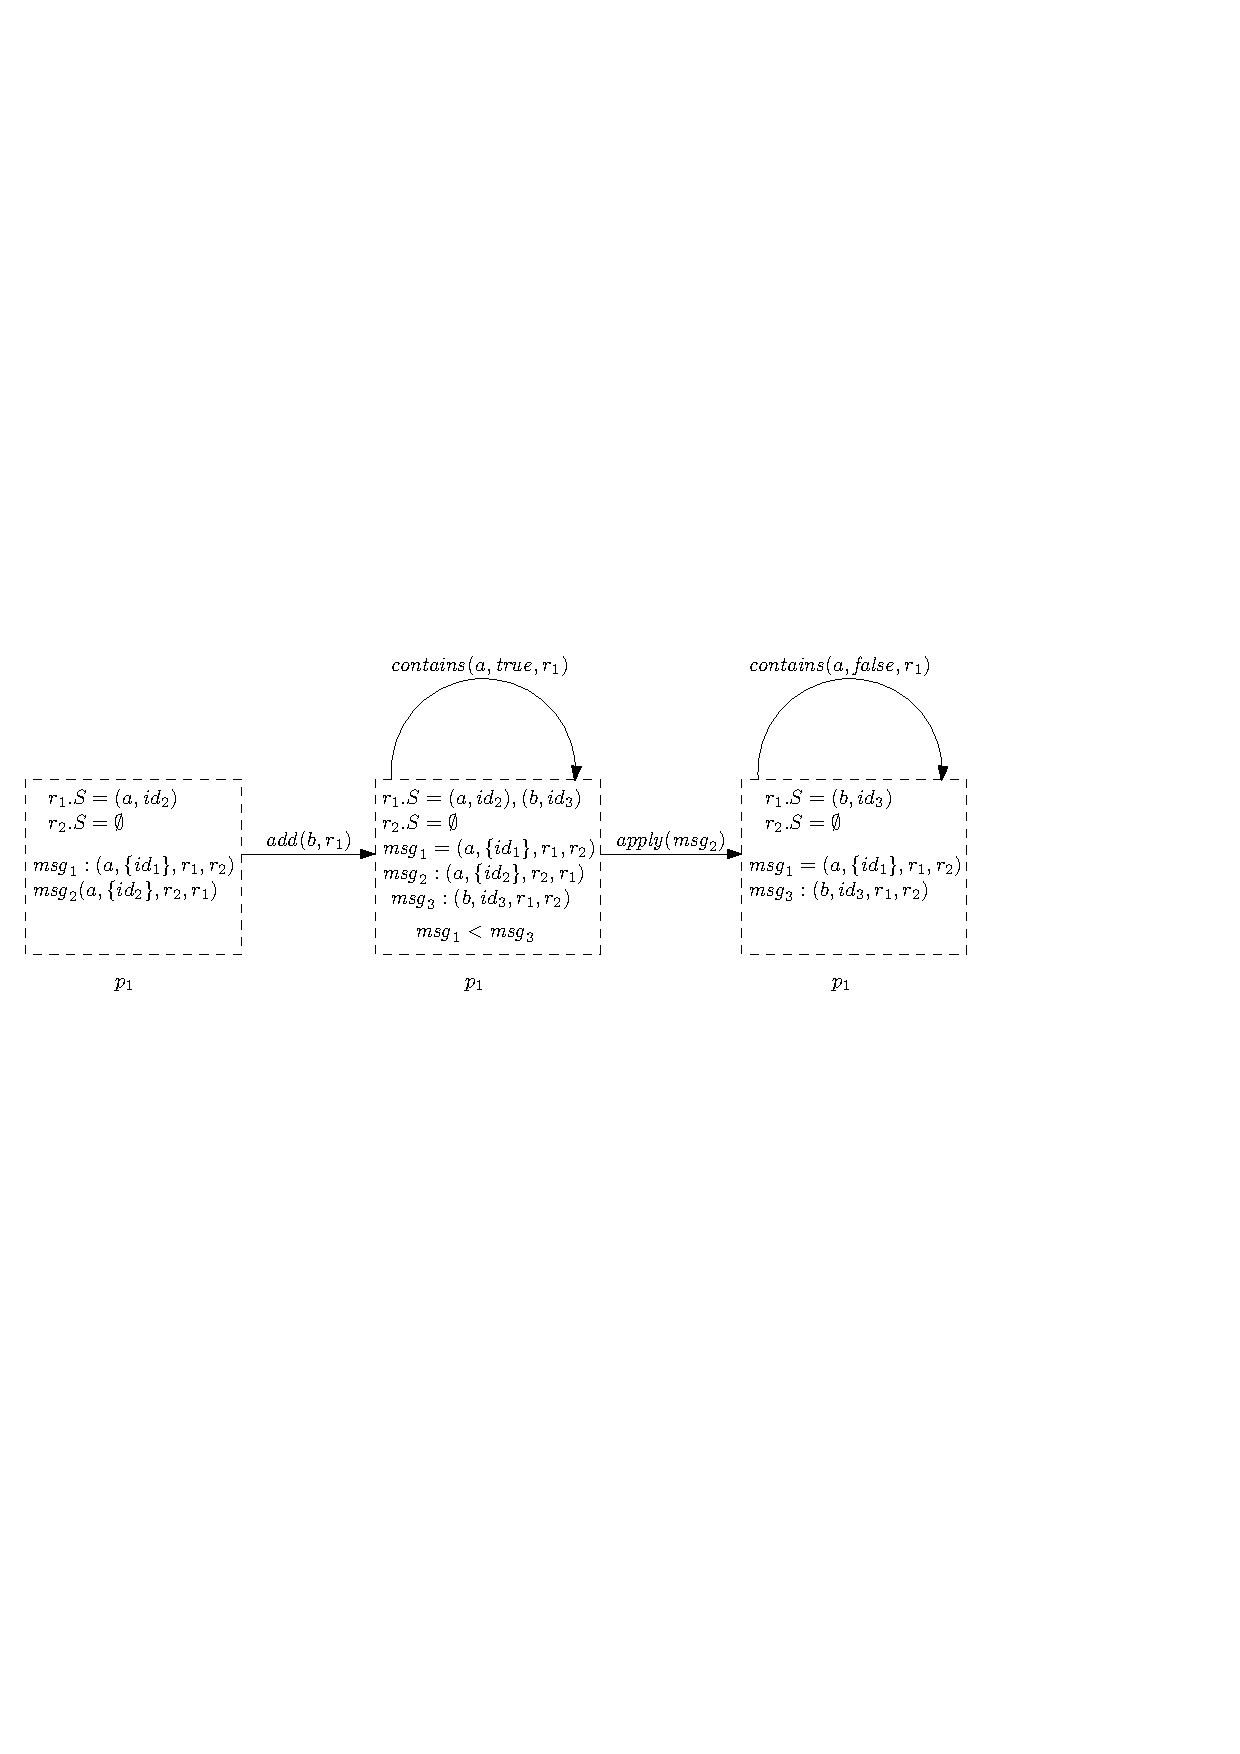
\includegraphics[width=0.8 \textwidth]{figures/PIC-OR-set-Implementation-Execution.pdf}
%\vspace{-10pt}
  \caption{OR-set implementation for \figurename~\ref{fig:succinct reference implementation for OR-set}.}
  \label{fig:or-set implemtation for succinct or-set specification}
\end{figure}

{\color {red}\figurename~\ref{fig:or-set implemtation for succinct or-set specification} gives the states of OR-set implementation that simulate states of specification in \figurename~\ref{fig:succinct reference implementation for OR-set}. State $p_1$, $p_2$ and $p_3$ simulates states $q'_1$, $q'_2$ and $q'_3$ of \figurename~\ref{fig:succinct reference implementation for OR-set}, respectively. To explain $(p_1,q'_1) \in R_{\mathit{sim}}$, we choose $(a,\mathit{id}_1)$ to be redundant, and $f$ maps $(a,\mathit{id}_2)$ into $+a_2$ and maps $(a,\{ \mathit{id}_2 \},r_2)$ into $-a_2$. This $f$ satisfies the requirements for message, $\mathit{FstRem}$ and visibility. To deal with the transitions from $p_1$ to $p_2$, we extend $f$ to additionally maps $(b,\mathit{id}_3)$ into $+b$, and put $(\mathit{msg}_1,\mathit{msg}_3)$ into $\mathit{msghb}$ to record the operation of $(a_1,\{ \mathit{id}_1 \},r_1)$ happens before the operation of $(b,\mathit{id}_3)$. Then it is easy to see that $(p_2,q'_2) \in R_{\mathit{sim}}$. To deal with the transitions from $p_2$ to $p_3$, we translate $\mathit{addDel}(-a_2,r_1)$ into $\mathit{msg}_2$. In $p_3$, $(a,\mathit{id}_1)$ and $(a,\mathit{id}_2)$ are both redundant, and $f$ maps $(b,\mathit{id}_3)$ into $+b$. Then it is easy to see $(p_3,q'_3) \in R_{\mathit{sim}}$.

Let us explain how to construct function $f_s$. $f_s$ is used to translate implementation transition label into specification transition label. It uses function $f$ to find operation of a message and to construct arbitration order. It ignores translating applying message of redundant operations. Formally, given implementation state $q_{\mathit{imp}}$, specification state $q_s$, where $(q_{\mathit{imp}},q_s) \in R_{\mathit{sim}}$, $f$ is the map between $\Sigma_e$ of $q_{\mathit{imp}}$ and operations of $q_s$, and $q_{\mathit{imp}} {\xrightarrow{\alpha}} q'_{\mathit{imp}}$. Then,

\begin{itemize}
\setlength{\itemsep}{0.5pt}
\item[-] $\alpha = apply(m)$: Let $m$ be message of $x \in \Sigma_e$. If $x$ is redundant, then $f_s(q_{\mathit{imp}},q_s,\alpha) = \epsilon$; Else, $f_s(q_{\mathit{imp}},q_s,\alpha) = addDel(f(x),r)$, where $r$ is the destination replica of $m$.

\item[-] $\alpha = (m,a,b,r,\mathit{arb}_{\mathit{imp}})$: $f_s(q_{\mathit{imp}},q_s,\alpha) = (m,a,b,r,\mathit{arb}'_s)$. If $m \in \mathbb{Q} \cup \{ \mathit{rem} \}$, then $\mathit{arb}'_s$ is same as the arbitration order of $q_s$; Else, assume the arbitration of $q'_{\mathit{imp}}$ is obtained from that of $q'_{\mathit{imp}}$ by inserting a new element in the $k$-th position, then $\mathit{arb}'_s$ is obtained from the arbitration order of $q_s$ by inserting $o$ at the $k$-th position, where $o=(m(a)\Rightarrow b,r,)$ is the unique possible operation for newly generated $m(a)\Rightarrow b$.
\end{itemize}

Here we implicitly assume that, when we comes to a pair of states, we change $f$ by only inserting or removing pairs of operations, not by changing existing pairs of operations. Given a trace $t = \alpha_1 \cdot \ldots \cdot \alpha_k$ of $\mathit{Sem}(\mathit{imp})$, function $f_t(t) = \beta_k$ works as follows: From the initial states $q_0^{\mathit{imp}}$ of $\mathit{Sem}(\mathit{imp})$, the initial state $q_0^{s}$ of $\mathit{SRImp}(\mathit{Spec})$, and $\alpha_1$, work as $f_s$ to obtain transition label $\beta_1$ and a new state $q_q^{s}$ of $\mathit{SRImp}(\mathit{Spec})$, and so on. The detailed definition can be found in Appendix \ref{sec:appendix definitions and proofs of section simulation and refinement}. It is easy to see that functions $f_s$ and $f_t$ hold as required.
}



%\subsection{Collection Specification without Causal Delivery}
%\label{subsec:collection specification without calusal delivery}

%In this subsection, we sketch the simulation relation for woot algorithm. The other part is similar to above subsection. For woot algorithm, $(q_{\mathit{imp}},q_s) \in R_{\mathit{sim}}$, if

Let us sketch the simulation relation for RGA. $(q_{\mathit{imp}},q_s) \in R_{\mathit{sim}}$, if

\begin{itemize}
\setlength{\itemsep}{0.5pt}
\item[-] An inductive invariant: For each replica $r$, the union of $\mathit{data}[r].N$ should form a TI tree, which are consistent with the TI tree of each replica. And the identifier in $\mathit{data}[r].T$ is a subset of that in $\mathit{data}[r].N$.

\item[-] An $\mathit{add}(a)$ is redundant, if for each replica $r$, identifier $a$ is in both $\mathit{data}[r].N$ and $\mathit{data}[r].T$.

\item[-] $f$ maps $(\mathit{add},a,t)$ into $\mathit{add}(a)$, and maps $(\mathit{rem},a,r)$ into $\mathit{rem}(a)$. This map preserves replica.

\item[-] Recognize the $\mathit{FstRem}$ relations: For each $a$, $f((\mathit{rem},a,\_)) \in \mathit{FstRem}(\mathit{add}(a))$. For each $b \neq a$, $f((\mathit{rem},b,\_)) \notin \mathit{FstRem}(\mathit{add}(a))$.

\item[-] Recognize the visibility relation: $(a,t,p) \in \mathit{data}[r].N$, if and only if $f((\mathit{add},a,t)) \in \mathit{visTo}(O,r,\mathit{vis})$. $a \in \mathit{data}[r].T$, if and only if there exists $(a,t,p)$ and $o_r$, such that $f((\mathit{add},a,t)) \in \mathit{visTo}(O,r,\mathit{vis})$, $o_r \in \mathit{FstRem}(f((\mathit{add},a,t)))$, and $o_r \in \mathit{visTo}(O,r,\mathit{vis})$.

\item[-] Arbitration order: We require that the arbitration order of $q_s$ is a sub-sequence of $f(f_{\mathit{arb}}(data,msgs))$.
\end{itemize}






















































\forget{
%An labeled transition system (LTS, for short) is a tuple $A = (Q,\Sigma,\rightarrow,q_0)$, where $Q$ is a set of states, $\Sigma$ is an alphabet of transition labels, $\rightarrow \subseteq Q \times \Sigma \times Q$ is a transition relation and $q_0$ is the initial state. A execution of $A$ is a sequences of transitions and states starting from the initial state $q_0$, and a trace is a sequence of transition labels of an execution. We say that $A$ is deterministic, if for each state $q$ and each transition label $\alpha$, $q$ has at most one $\rightarrow$ successor with transition label $\alpha$.



%A execution of $A$ is a sequence $\alpha_1 \cdot \ldots \cdot \alpha_k \in \Sigma^*$, such that $\exists q_1,\ldots,q_k \in Q$, $q_0 {\xrightarrow{\alpha_1}} q_1 \ldots {\xrightarrow{\alpha_k}} q_k$. We say that $A$ is deterministic, if $\forall q \in Q$ and $\forall \alpha \in \Sigma$, there exists at most one $q' \in Q$, such that $q {\xrightarrow{\alpha}} q'$.

%\todo{Define execution as $q_0 {\xrightarrow{\alpha_1}} q_1 \ldots {\xrightarrow{\alpha_k}} q_k$ and trace as $\alpha_1 \cdot \ldots \cdot \alpha_k$, extracted from an execution. Extend the notation $\xrightarrow{\alpha_1}$ to words instead of letters.}

%\todo{Don't use $\forall$ and $\exists$ in a textual description, but only in formulas}

Given two LTS $A_1 = (Q_1,\Sigma_1,\rightarrow_1,q_{0}^1)$ and $A_2 = (Q_2,\Sigma_2,\rightarrow_2,q_{0}^2)$ and two functions $f_s: Q_1 \times Q_2 \times \Sigma_1 \rightarrow \Sigma_2$ and $f_t:\Sigma_1^* \rightarrow \Sigma_2$, we define our simulation and refinement relations as follows:

%Given two LTS $A = (Q_A,\Sigma_A,\rightarrow_A,q_{0A})$ and $B = (Q_B,\Sigma_B,\rightarrow_B,q_{0B})$ with alphabet $\Sigma_A$ and $\Sigma_B$, respectively. Given functions $f_s: Q_A \times Q_B \times \Sigma_A \rightarrow \Sigma_B$ and $f_t:\Sigma_A^* \rightarrow \Sigma_B$, we define our simulation and refinement relations as follows:

%\todo{Use $A_1$ and $A_2$ instead of $A$ and $B$, so that all the components are indexed by 1,2, except for $q_0$ which becomes $q_0^{1/2}$.}

\begin{definition}[$f_s$-Simulation]
\label{definition:fs simulation}
Relation $R \subseteq Q_1 \times Q_2$ is a $f_s$-simulation relation, if whenever $(q_1,q_2) \in R \wedge q_1 {\xrightarrow{\alpha}}_1 q'_1$,
%A $f_s$-simulation relation $R \subseteq Q_A \times Q_B$ is a relation that satisfies: If $(q_a,q_b) \in R \wedge q_a {\xrightarrow{\alpha}}_A q'_a$ for some $q_a$, then
\begin{itemize}
\setlength{\itemsep}{0.5pt}
\item[-] If $f_s(q_1,q_2,\alpha) \neq \epsilon$, then $q_2 {\xrightarrow{f_s(q_1,q_2,\alpha)}}_1 q'_2 \wedge (q'_1,q'_2) \in R$.

\item[-] If $f_s(q_1,q_2,\alpha) = \epsilon$, then $(q'_1,q_2) \in R$.
\end{itemize}
\end{definition}

%\todo{Again, use indexing with 1,2}

\begin{definition}[refinement w.r.t $f_t$]
\label{definition:ft refinement}
$A_2$ refines $A_1$ w.r.t $f_t$, if for each trace $t_1 = \alpha_1 \cdot \ldots \cdot \alpha_k$ of $A_1$, $t_2 = f_t(\alpha_1) \cdot \ldots \cdot f_t(\alpha_1 \cdot \ldots \cdot \alpha_k)$ is an execution of $A_2$.
\end{definition}

%\todo{$B$ $f_t$-refines $A$ to be rewritten to ``$B$ refines $A$ w.r.t. $f_t$''}

%\todo{Give a name to the property $P_{(f_s,f_t)}$, for instance: we say that $f_s$ and $f_t$ are compatible ... }

We say that $f_s$ and $f_t$ are compatible, if for each deterministic $A_2$, the following holds: For each execution %\todo{execution}
$q_{0}^1 {\xrightarrow{\alpha_1}}_1 q_{1}^1 \ldots {\xrightarrow{\alpha_k}}_1 q_{k}^1$ of $A_1$ and each $1 \leq u \leq k$, we have $f_t(\alpha_1 \cdot \ldots \cdot \alpha_{u+1}) = f_s(q_{u}^1,q_{u}^2,\alpha_{u+1})$, here $q_u^2$ is a state obtained by $q_{0}^2 {\xrightarrow{f_t(\alpha_1) \cdot \ldots \cdot f_t(\alpha_1 \cdot \ldots \cdot \alpha_u) }}_2 q_u^2$. %\todo{write it explicitly using the extension of $\xrightarrow{\alpha_1}$ to words}
The following theorem states that $f_s$ and $f_t$ are compatible, $f_s$-simulation is equivalent to refinement w.r.t $f_t$. Its proof can be found in Appendix \ref{sec:appendix definitions and proofs of section simulation and refinement} and is similar to that in \cite{Abadi:1991,Lynch:1995}.

%If $B$ is deterministic, then we defined a property $P_{(f_s,f_t)}$ as follows: For each transitions \todo{execution} $q_{0A} {\xrightarrow{\alpha_1}}$ $q_{1A} \ldots {\xrightarrow{\alpha_k}} q_{kA}$ of $A$, $\forall 1 \leq i < k$, $f_t(\alpha_1 \cdot \ldots \cdot \alpha_i \cdot \alpha_{i+1}) = f_s(q_{iA},q_{iB},\alpha_{i+1})$, where $q_{iB}$ is obtained from $q_{0B}$ by doing $f_t(\alpha_1) \cdot \ldots \cdot f_t(\alpha_1 \cdot \ldots \cdot \alpha_i)$ transitions \todo{write it explicitly using the extension of $\xrightarrow{\alpha_1}$ to words}. The following theorem states that when $P_{(f_s,f_t)}$ holds, $f_s$-simulation is equivalent to $f_t$-refinement. Its proof can be found in Appendix \ref{sec:appendix definitions and proofs of section simulation and refinement} and is similar to that in \cite{Abadi:1991,Lynch:1995}.

\begin{theorem}
\label{theorem:equivalence of our simulation and refinement}
Given an LTS $A_1$ and a deterministic LTS $A_2$ and functions $f_s,f_t$, such that $f_s$ and $f_t$ are compatible. $A_2$ refines $A_1$ w.r.t $f_t$, if and only if there exists a $f_s$-simulation relation between $A_1$ and $A_2$.
\end{theorem}
}







\forget
{
\section{Simulation Relation}
\label{sec:simulation relation}

In this section, we give our simulation relation between a implementation $\llbracket imp \rrbracket$ and a reference implementation (with causal delivery) $A$. For plus-minus specification and its compacted reference implementation $A'$, we give our simulation relation between $\llbracket imp \rrbracket$ and $A'$. For both simulation relations, we prove that they are sound and complete for refinement checking.

Given $\llbracket imp \rrbracket = (Q_{imp},\Sigma_{imp},\rightarrow_{imp},q_{0imp})$ and $RImp(Spec) = (Q_s,\Sigma_s,vis,q_{0s},li,\rightarrow_s,livReq)$, we say that $R \subseteq Q_{imp} \times Q_s$ is a simulation relation, if given $(q_i,q_s) \in R$

\begin{itemize}
\setlength{\itemsep}{0.5pt}
\item[-] If $q_i {\xrightarrow{m(a,b,r)}}_{imp} q'_i$, then $q_s {\xrightarrow{m(a,b,r)}}_s q'_s$ and $(q'_i,q'_s) \in R$.

\item[-] If $q_i {\xrightarrow{apply(m)}}_{imp} q'_i$, then $q_s {\xrightarrow{addDel(o,r)}}_s q'_s$ and $(q'_i,q'_s) \in R$. Here $o$ and $r$ are obtained as follows: Assume $m=(\_,r',r)$ is the $i-th$ among messages of $q_i$ with source replica $r'$ and destination replica $r$ w.r.t $<_{sd}$. Then, $o$ is the $i-th$ among operations of $q_s$ which happens on replica $r'$ and not visible to replica $r$ w.r.t $ro$.
\end{itemize}




\forget{
Given $\llbracket imp \rrbracket = (Q_{imp},\Sigma_{imp},\rightarrow_{imp},q_{0imp})$ (not assuming causal delivery) and $RImp(Spec) = (Q_s,\Sigma_s,vis,q_{0s},li,\rightarrow_s,livReq)$, we say that $R \subseteq Q_{imp} \times Q_s$ is a simulation relation, if given $(q_i,q_s) \in R$ where $q_i = (repD,msgs,<_{roi})$ and $q_s = (uO,ro,del)$,

\begin{itemize}
\setlength{\itemsep}{0.5pt}
\item[-] Let $MsgToOp(q_i) = \{ o \vert \exists m = (dat,\_,\_) \in msgs, o=op(dat) \}$ be the set of operations of messages in $q_i$. Let $AOpS(q_s) = \{ o \vert o \in uO, \exists r, \neg (o {\xrightarrow{vis}} r) \}$ be the set of operations in $q_s$ that are not delivered into all replicas. Given $r \in RId$, let $MsgToOp(q_i)(r) = \{ o \vert \exists m = (dat,\_,r) \in msgs, o=op(dat) \}$ and $AOpS(q_s)(r) = \{ o \vert o \in uO, \neg (o {\xrightarrow{vis}} r) \}$. We require that,

    \begin{itemize}
    \setlength{\itemsep}{0.5pt}
    \item[-] $\forall r \in RId$, $\vert MsgToOp(q_i)(r) \vert = \vert AOpS(q_s)(r) \vert$.

    \item[-] There is a function $f_{(q_i,q_s)}$ that maps the $i-th$ op of $MsgToOp(q_i)(r)$ w.r.t $<_{roi}$ into the $i-th$ op of $AOpS(q_s)(r)$ w.r.t $ro$ for each $i$. Moreover, $o_1 = OpMsgI(q_i)(r_1)$, $o_2 = OpMsgI(q_i)(r_2)$, $r_1 \neq r_2$, and $o_1$ and $o_2$ are mapped from same $dat$, if and only if $f_{(q_i,q_s)}(o_1)=f_{(q_i,q_s)}(o_2)$. We can see that such $f_{(q_i,q_s)}$ is unique if it exists.
    \end{itemize}

\item[-] If $q_i {\xrightarrow{m(a,b,r)}}_{imp} q'_i$, then $q_s {\xrightarrow{m(a,b,r)}}_s q'_s$ and $(q'_i,q'_s)$.

\item[-] If $q_i {\xrightarrow{apply(m)}}_{imp} q'_i$, $m=(dat,\_,r)$ and $f_{(q_i,q_s)}(op(dat))=o$, then $q_s {\xrightarrow{addDel(o,r)}}_s q'_s$ and $(q'_i,q'_s)$.
\end{itemize}

}




We say that a transition system is deterministic, if for each state $q$ and transition label $\alpha$, from $q$ there is at most one transition with label $\alpha$. {\color {red}It is safe to assume that when constructing reference implementation $RImp(Spec)$, in update operation transitions $q_s {\xrightarrow{m(a,b,r)}}_s q'_s$, we permit only one possible identifier of the newly added operation of $q'_i$. For example, each replica has a counter for generating unique identifier of operations. In this way, it is obvious that $RImp(Spec)$ is deterministic.}

Given a sequence $t_{imp} = \alpha_1 \cdot \ldots \in \llbracket imp \rrbracket$ and a sequence $t_s = \beta_1 \cdot \ldots \in RImp(Spec)$, we say that $t_{imp}$ and $t_s$ correspond, if

\begin{itemize}
\setlength{\itemsep}{0.5pt}
\item[-] If $\alpha_i$ is an operation, then $\beta_i = \alpha_i$.

\item[-] Else, $\alpha_i = apply(m)$ and $\beta_i = addDel(o,r)$. Here $o$ and $r$ are obtained as follows: Assume after doing $\alpha_1 \cdot \ldots \cdot \alpha_{i-1}$, $m=(\_,r',r)$ is the $i-th$ among ``messages with source replica $r'$ and destination replica $r$ and still not applied'' w.r.t the occurring order of $t_{imp}$. {\color {red}Here we assume that in $\llbracket imp \rrbracket$, the set of newly generated messages could be seen as ghost variable of $m(a,b,r)$ transitions.}

    Then, after doing $\beta_1 \cdot \ldots \cdot \beta_{i-1}$, $o$ is the $i-th$ among ``operations which happens on replica $r'$ and not visible to replica $r$'' w.r.t the occurring order of $t_s$. {\color {red} Here we assume that in $RImp(Spec)$, the newly generated operation could be seen as ghost variable of $m(a,b,r)$ transitions.}
\end{itemize}

We can prove that, given $t_{imp}$, there exists at most one $t_s$, such that $t_{imp}$ and $t_s$ correspond. The reason is that, (1) $RImp(Spec)$ is deterministic, and (2) to deal with $apply(m)$ transition, there is only one possible selection of operation $o$.

We say that $RImp(Spec)$ trace refines $\llbracket imp \rrbracket$, if $\forall t_{imp} \in \llbracket imp \rrbracket$, $\exists t_s \in RImp(Spec)$, such that $t_{imp}$ and $t_s$ correspond. It is obvious that our simulation relation implies trace inclusion. Since $RImp(Spec)$ is deterministic, similarly as that of \cite{Abadi:1991,Lynch:1995}, we could prove that the opposite direction also holds. Therefore, our simulation relation is a sound and complete method to prove trace refinement, as states by the following theorem:

\begin{theorem}
\label{theorem:equivalence of our simulation relation and sequence inclusion}
$RImp(Spec)$ trace refines $\llbracket imp \rrbracket$, if and only if there exists a simulation relation between $\llbracket imp \rrbracket$ and $RImp(Spec)$.
\end{theorem}



When we consider implementation and reference implementation with causal delivery, above definitions and lemmas still hold. The reason is that, we could easily obtain $<_{sd}$ order from $<$ order in state of implementation.




\subsection{Simulation Relation for Plus-Minus Specification}
\label{subsec:simulation relation for plus-minus specification}

Let $\llbracket imp \rrbracket_{pm}$ be obtained from $\llbracket imp \rrbracket$ by making applying of some messages invisible. Formally,

\begin{itemize}
\setlength{\itemsep}{0.5pt}
\item[-] Each state is of the form $(repD,msgs,<_{sd})$. We change $msgs$ such that there are two kinds of messages: $(dat,r,r')$ and $(data,r,r')_{inv}$.

\item[-] $\Sigma = \{ \epsilon, m(a,b,r), apply(msg) \vert m \in M, a,b \in D, r \in RId, msg \in Msg \}$ is the set of transition labels.

\item[-] When doing operation transitions, some message is transformed into invisible. For example, if $(redD,msgs,<_{sd}) {\xrightarrow{m(a,b,r)}} (redD',msgs',<'_{sd})$ is a transition of $\llbracket imp \rrbracket$, then $(redD,msgs,<_{sd}) {\xrightarrow{m(a,b,r)}} (redD',f(msgs'),<'_{sd})$ is a transition of $\llbracket imp \rrbracket_{pm}$. Here $f(msgs')$ is obtained from $msgs'$ by adding subfix $inv$ into some messages.
\item[-] When applying a message $(\_,\_,\_)$, same as before.

When applying a message $(\_,\_,\_)_{inv}$, use $\epsilon$ as transition label.
\end{itemize}


Given $\llbracket imp \rrbracket_{pm} = (Q_{imp},\Sigma_{imp},\rightarrow_{imp},q_{0imp})$ and $CRImp(Spec) = (Q_s,\Sigma_s,vis,q_{0s},li,\rightarrow_s,livReq)$, we say that $R \subseteq Q_{imp} \times Q_s$ is a weak simulation relation, if given $(q_i,q_s) \in R$

\begin{itemize}
\setlength{\itemsep}{0.5pt}
\item[-] If $q_i {\xrightarrow{m(a,b,r)}}_{imp} q'_i$, then $q_s {\xrightarrow{m(a,b,r)}}_s q'_s$ and $(q'_i,q'_s) \in R$.

\item[-] If $q_i {\xrightarrow{apply(m)}}_{imp} q'_i$, $m=(\_,r',r)$, then $q_s {\xrightarrow{addDel(o,r)}}_s q'_s$ and $(q'_i,q'_s) \in R$. Here $o$ is obtained as follows: Assume $m$ is the $i-th$ among messages of $q_i$ with source replica $r'$, destination replica $r$ and are visible w.r.t $<_{sd}$. Then, $o$ is the $i-th$ among operations of $q_s$ which happens on replica $r'$ and not visible to replica $r$ w.r.t $ro$.

\item[-] If $q_i {\xrightarrow{apply(m)}}_{imp} q'_i$, $m=(\_,r',r)_{inv}$, then $(q'_i,q_s) \in R$.
\end{itemize}


Given a sequence $t_{imp} = \alpha_1 \cdot \ldots \in \llbracket imp \rrbracket_{pl}$ and a sequence $t_s = \beta_1 \cdot \ldots \in CRImp(Spec)$, we say that $t_{imp}$ and $t_s$ correspond, if

\begin{itemize}
\setlength{\itemsep}{0.5pt}
\item[-] If $\alpha_i$ is an operation, then $\beta_i = \alpha_i$.

\item[-] Else, if $\alpha_i = apply(m=(\_,r',r))$ and $\beta_i = addDel(o,r)$. Here $o$ is obtained as follows: Assume after doing $\alpha_1 \cdot \ldots \cdot \alpha_{i-1}$, $m$ is the $i-th$ among ``messages with source replica $r'$ and destination replica $r$ and still not applied and are visible'' w.r.t the occurring order of $t_{imp}$. Then, after doing $\beta_1 \cdot \ldots \cdot \beta_{i-1}$, $o$ is the $i-th$ among ``operations which happens on replica $r'$ and not visible to replica $r$'' w.r.t the occurring order of $t_s$.

\item[-] Else, $\alpha_i = apply(m=(\_,r',r)_{inv})$ and $\beta_i = \epsilon$.
\end{itemize}

We say that $CRImp(Spec)$ weak trace refines $\llbracket imp \rrbracket_{pl}$, if $\forall t_{imp} \in \llbracket imp \rrbracket_{pl}$, $\exists t_s \in CRImp(Spec)$, such that $t_{imp}$ and $t_s$ correspond. It is obvious that our weak simulation relation implies trace inclusion. Since $RImp(Spec)$ is deterministic, similarly as that of \cite{Abadi:1991,Lynch:1995}, we could prove that the opposite direction also holds. Therefore, our weak simulation relation is a sound and complete method to prove trace refinement, as states by the following theorem:

\begin{theorem}
\label{theorem:equivalence of our simulation relation and sequence inclusion for add-plus specification and its compacted reference implementation}
$CRImp(Spec)$ trace refines $\llbracket imp \rrbracket_{pl}$, if and only if there exists a weak simulation relation between $\llbracket imp \rrbracket_{pl}$ and $CRImp(Spec)$.
\end{theorem}
}

